In this section we discuss the goals we follow in building \projectname.
We then present the architectural details of our prototype implementation~\cite{prototype}
and discuss the particular implementation challenges.

\subsection{Implementation Goals: The 7 rules of \projectname{}}

The main focus of our system is to be able to study failure modes and corner
cases prevalent in large-scale, production topologies. As such, our solution
should scale to network sizes found in production data-centers today,~e.g.,
$1,000$ to $10,000$ switches and $20,000$ to $100,000$ end-hosts. Today, such
topologies typically are managed with \emph{proactive} rules, for performance
predictability and due to hardware constraints. As such, we don't need to focus
on precise simulation of \emph{data-plane} traffic, but rather on \emph{control
plane events} induced by host, link and switch failures, and topology changes,
as induced,~e.g., by virtual machine migrations. Our implementation goals are
thus:

\textbf{(1) Scalability} 
We require our simulator to scale up to large topology sizes,
e.g., a Fat-Tree topology~\cite{fattree} with 48 pods. 

\textbf{(2) Control plane focus} We expect the dynamism in our system to stem from
\emph{control plane events}. Typical rates of control plane events must thus be
handled, and control plane events must be modeled precisely. Conversely, we
don't expect to handle a realistic amount of dataplane traffic, which is
intractable for a software solution, and largely irrelevant in current networks.

\textbf{(3) Controller choice} Our system should run with existing production
controllers with minimum instrumentation. We don't want to limit ourselves to
a particular controller/NOS implementation,.

\textbf{(4) Full determinism} We want our simulation environment to be fully 
deterministic, such that repeated simulations with identical initialization values
yield provably identical results. This creates a challenge in conjunction with our goal (3).

\textbf{(5) Failure Modes} The system should model failure modes and critical conditions
accurately, including switch and link failures, message drops, delays reordering (where possible).

\textbf{(6) Corner cases investigation} The potential state-space in a large-scale network
is intractably large. We focus on interesting cases, as recorded, e.g., in production, or
found through interactive evaluation. To investigate related error conditions,
we \emph{fuzz} the input traces.

\textbf{(7) Interactivity} We system should fast enough for interactive exploration through
an operator.

\subsection{Architecture}

We now discuss the architecture of \projectname in detail and discuss how it
relates to the goals outlined in the last section. Figure \ref{fig:system}
depicts our architecture. We address the parts in turn:

\begin{figure*}[!t]
  \centering
  \includegraphics[width=0.8\textwidth]{../diagrams/architecture/architecture.pdf}
  \caption{System architecture}
  \label{fig:system}
\end{figure*}

\noindent{\bf Trace Input And Fuzzing} Event generation has two components.
We first generate system executions, which come from one of three sources:
\begin{enumerate}
  \item \emph{traces taken from the real networks.} This enables us to investigate 
  real-world bugs in a controlled lab environment. For collecting traces,
  we use OFRewind~\cite{ofrewind} and related systems.
\item \emph{synthetic traces.} We also generate synthetic traces for our anlaysis
  based on a simple model for network failures and other sources of control plane
  events.
\item \emph{model checking} Model checking and codepath analysis of parts of the
  controller systems represents another opportunity for generating input traces
  that exercise interesting corner case behavior. Note that due to the large network
  size, we consider a full exploration of the state
  space to be intractable.
\item \emph{interactive} Lastly, the troubleshooter can manually inject events into
  the network. This if the troubleshooter already has an intuition of what might be
  the trigger event sequence.
\end{enumerate}

To locate the minimum trigger sequence of policy-violation as described in
\S\ref{sec:approach}, we repeatedly execute the system over the same event sequence,
while \emph{sub-selecting} events.

\noindent{\bf Simulator} The main simulator is modeled as a single,
deterministic python process. Switches are emulated as lightweight python
objects.\footnote{In contrast to common software switches like
OpenVSwitch~\cite{openvswitch} these switches are optimized for precise,
controllable emulation of hardware control-plane behavior, not data-plane
forwarding speed.} The controllers are spawned as separate processes and
communicate with the emulated switches through normal TCP sockets via the
OpenFlow protocol. The IO-logic is based on an event-based worker model and
scales up to $>10,000$ switches through the use of optimized select primitives
like \texttt{epoll}.

The simulation proceeds in discrete timesteps. In each timestep, events are
sourced from the configured event sources and injected into the system. To
simulate delays on the control plane, e.g., through packet loss or queuing of
control plane packets, the simulator maintains a pair of buffers for each
OpenFlow connection. It controls when OpenFlow messages reach the processing
logic within the simulator.

\noindent{\bf Controller Sandbox}
Our goals of being able to run arbitrary controllers on top of our simulator
and being able to reproduce runs deterministically creates the challenge
of creating a reproducible environment for the controllers. We address this
challenge by running the guest controllers in a sandbox. The sandbox is 
orchestrated and controlled by the main simulator processes and limits
the visibility of external non-deterministic events to the controller (e.g.,
sources of randomness, timers).

There are a number of implementation options for the sandbox, that form a
trade-off between generality and performance of the solution. The options
include (i) \emph{software-layer instrumenation} -- replacing timer methods and
random generator-method in the controller with deterministic versions that are
controlled by the main simulator (ii) \emph{language runtime instrumentation}
modern language runtimes like the JVM offer the possibility to instrument and
control the runtime via plugins. The provides lightweight determinism without
the need for modifying the controller application itself. (iii) \emph{Binary
instrumentation} there exist several solutions that enable determinism based on
binary instrumentation~\cite{XXX}. These must deal with lower-level events and
thus exhibit a higher overhead than runtime-specific instrumentation, but offer
the opportunity to instrument arbitrary language programs. (iv) \emph{Virtual machines}
Virtual machines can be used for achieving fully deterministic replay. The
offer the greatest accuracy, and generality but also the highest overhead.

For generality, by default, we run controllers in VMs. As the sandbox control
happens through normal TCP sockets, we can run controllers on dedicated machines
to avoid CPU or memory bottlenecks.

\noindent{\bf Correspondence Checking}

For multilayer correspondence checking, \projectname requires snapshots of the
network graph present in the network operating system at different layers. For this,
we use a simple request-response protocol and an extensible data serialization in
JSON that can be implemented with a small amount of code. For instance, we have
implemented the interface in the Floodlight controller in <500 LoC of Java.

The correspondence checking is performed by the HSA framework~\cite{hsa}, that
we modified for our purposes. \andi{@colin, describe the modifications and operation
mode of the correspondence checks.}
